%%% Содержимое слайдов

\frame[plain]{\titlepage} % Титульный слайд

%-------------------------------------------------------------------------------

\section{Разработка виртуальной инфраструктуры для реализации облачных услуг}

\begin{frame}
\frametitle{\insertsection}
Возможности: (стоит ли вообще иметь этот слайд? или как-то грамотно изменить его?)
\begin{itemize}
	\item финансовые ограничения
	\item единственный проектировщик
	\item отсутствие опыта работы с виртуализацией
	\item желание что-то построить
	\item ??? что-то еще упустил ???
\end{itemize}
\end{frame}

\begin{frame}
\frametitle{\insertsection}
Требования:
\begin{itemize}
	\item устранение единых точек отказа %(резервные линки, RAID)
	\item защита от несанкционированного доступа и атак %(DDoS, флуд)
	\item \textbf{использование свободного ПО (по возможности?? или перефразировать?)}
	\item документирование инфраструктуры
	\item автоматизация инфраструктуры
	\item разработка эффективных тарифных планов хостинга
	\item использование в бизнесе
\end{itemize}
\end{frame}

%-------------------------------------------------------------------------------

\section{Общая схема инфраструктуры}

\begin{frame}
\frametitle{\insertsection}
\begin{figure}[h]
	\begin{center}
		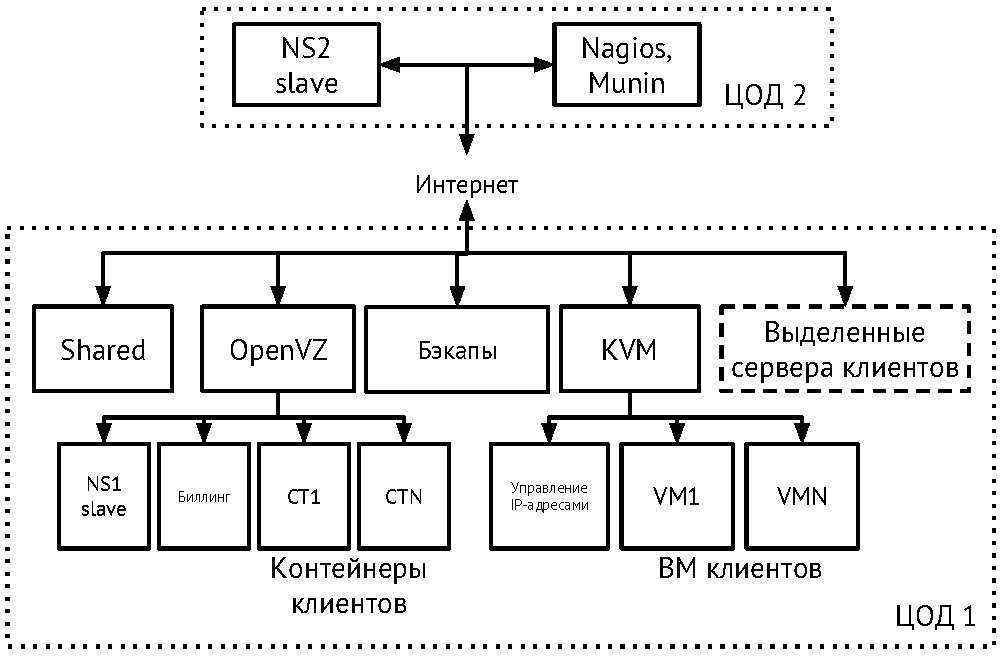
\includegraphics[width=\linewidth]{infrast-scheme}
	\end{center}
\end{figure}
\end{frame}

%-------------------------------------------------------------------------------

\section{Используемый инструментарий}

\begin{frame}
\frametitle{\insertsection}
\begin{itemize}
	\item ОС Linux
	\item мониторинг
	\item виртуализация
	\item автоматизированное управление конфигурациями
	\item скрипты, много скриптов (???)
	\item стандартный стек ПО хостинга
	\item защита от вредоносного ПО
	\item панели для пользователей виртуальных серверов
\end{itemize}
\end{frame}

%-------------------------------------------------------------------------------

\section{Операционная система}

\begin{frame}
\frametitle{\insertsection}
\framesubtitle{CentOS 7 (GPL)}
\begin{itemize}
	\item 494 из 500 крупнейших суперкомпьютеров работают на Linux
	\item (изобилие)? серверного ПО
	\item поддержка 6-10 лет (обновление пакетов, исправление уязвимостей и багов)
	\item бесплатно
	\item простая сборка пакетов
	\item драйвера
	\item много документации
\end{itemize}
\end{frame}

%-------------------------------------------------------------------------------

\section{Мониторинг}

\begin{frame}
\frametitle{\insertsection}
\framesubtitle{Nagios → Icinga2 (GPLv2)}
\begin{figure}[h]
	\begin{center}
		\begin{multicols}{2}
		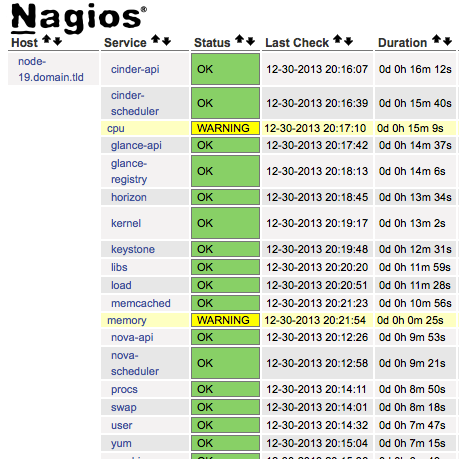
\includegraphics[width=\linewidth]{nagios} \pause \\
		\uncover<2->{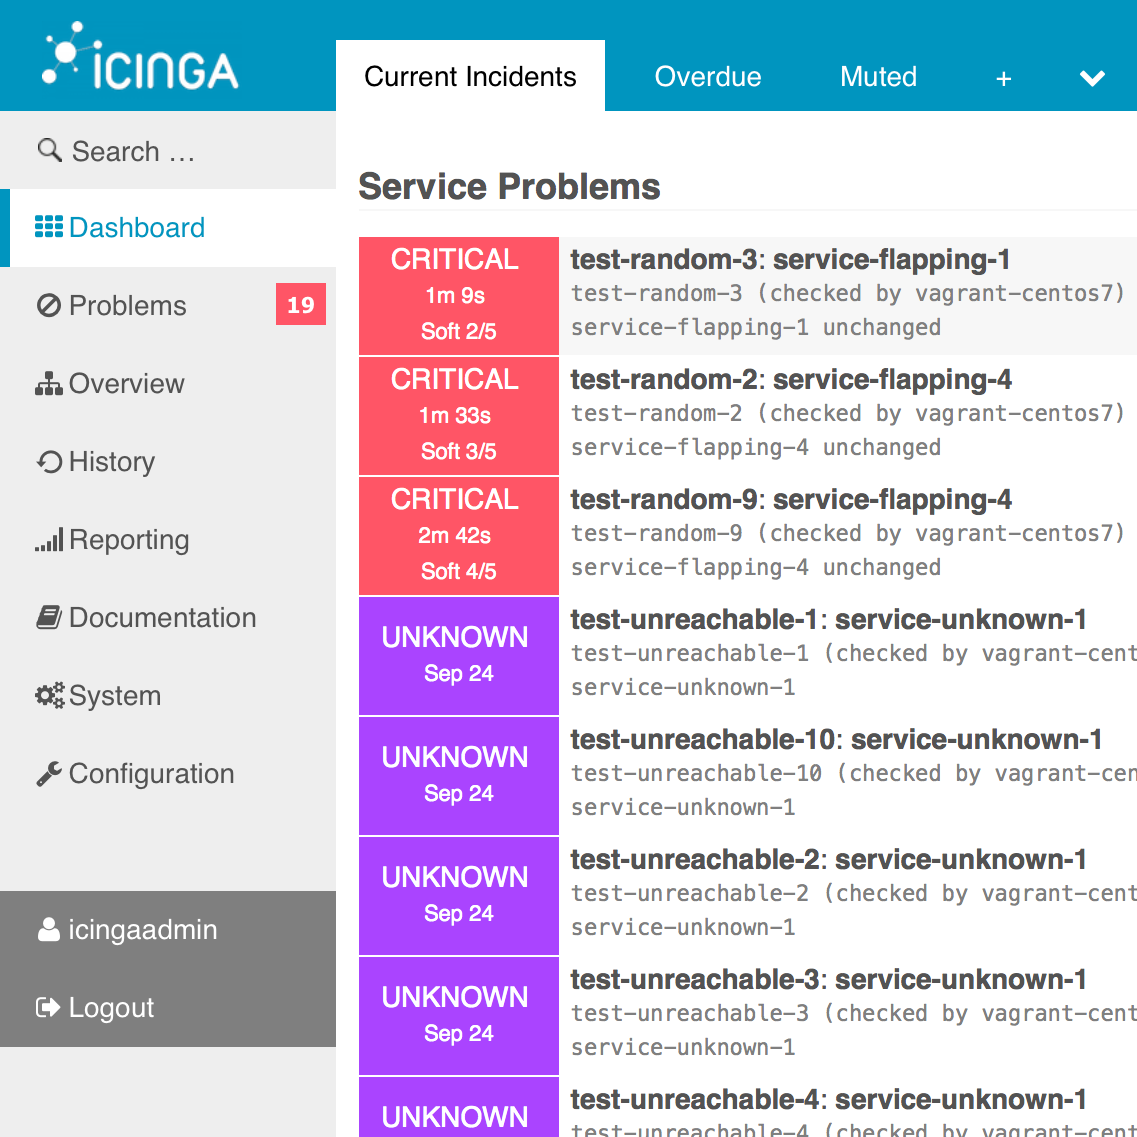
\includegraphics[width=\linewidth]{icinga2}}
		\end{multicols}
	\end{center}
\end{figure}
\end{frame}

%-------------------------------------------------------------------------------

\section{Метрики}

\begin{frame}
\frametitle{\insertsection}
\framesubtitle{Munin (GPL)}
\begin{figure}[h]
	\begin{center}
		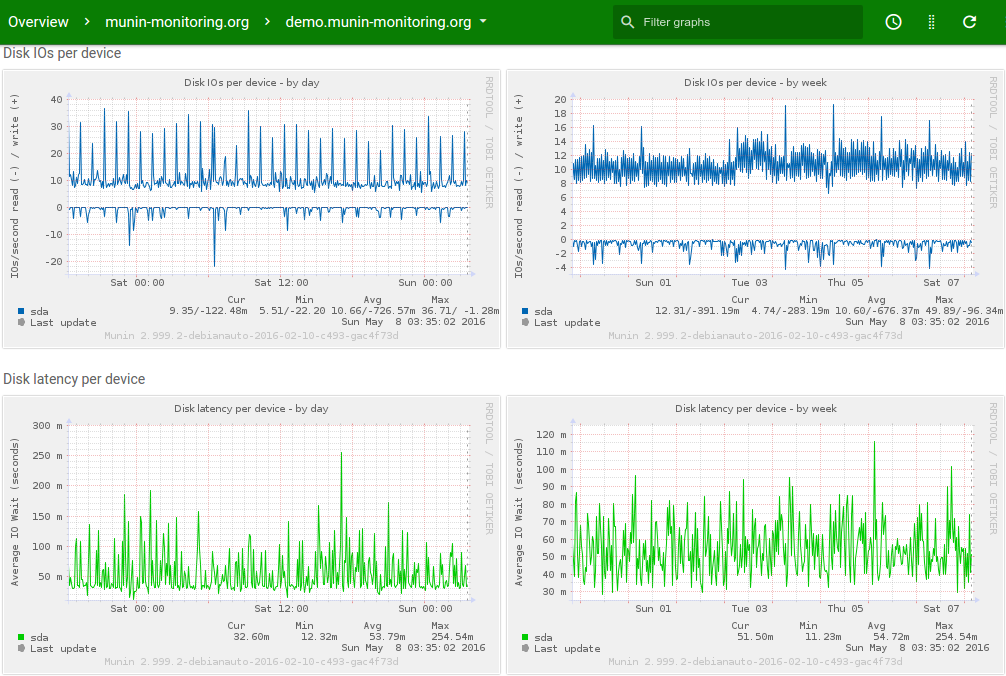
\includegraphics[width=\linewidth]{munin}
	\end{center}
\end{figure}
\end{frame}

%-------------------------------------------------------------------------------

\section{Автоматизация управления}

\begin{frame}
\frametitle{\insertsection}
\framesubtitle{Ansible (GPL) + git (GPLv2)}
\begin{figure}[h]
	\begin{center}
		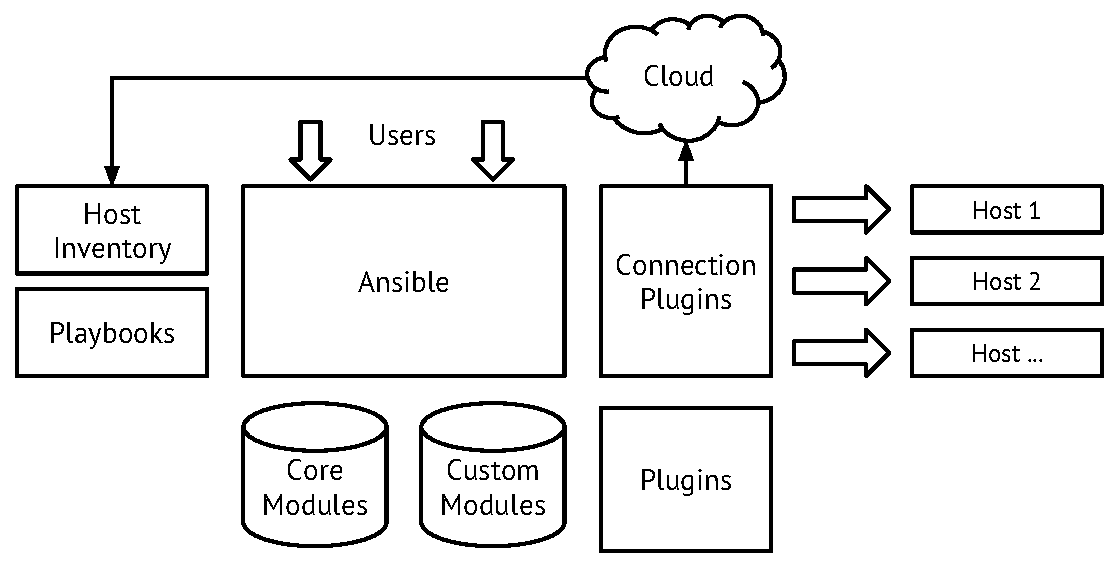
\includegraphics[width=\linewidth]{ansible}
	\end{center}
\end{figure}
\end{frame}

%-------------------------------------------------------------------------------

\section{Виртуализация}

\begin{frame}
\frametitle{\insertsection}
\framesubtitle{OpenVZ (GPLv2) + KVM (GPL/LGPL)}
\begin{figure}[h]
	\begin{center}
		\begin{multicols}{2}
		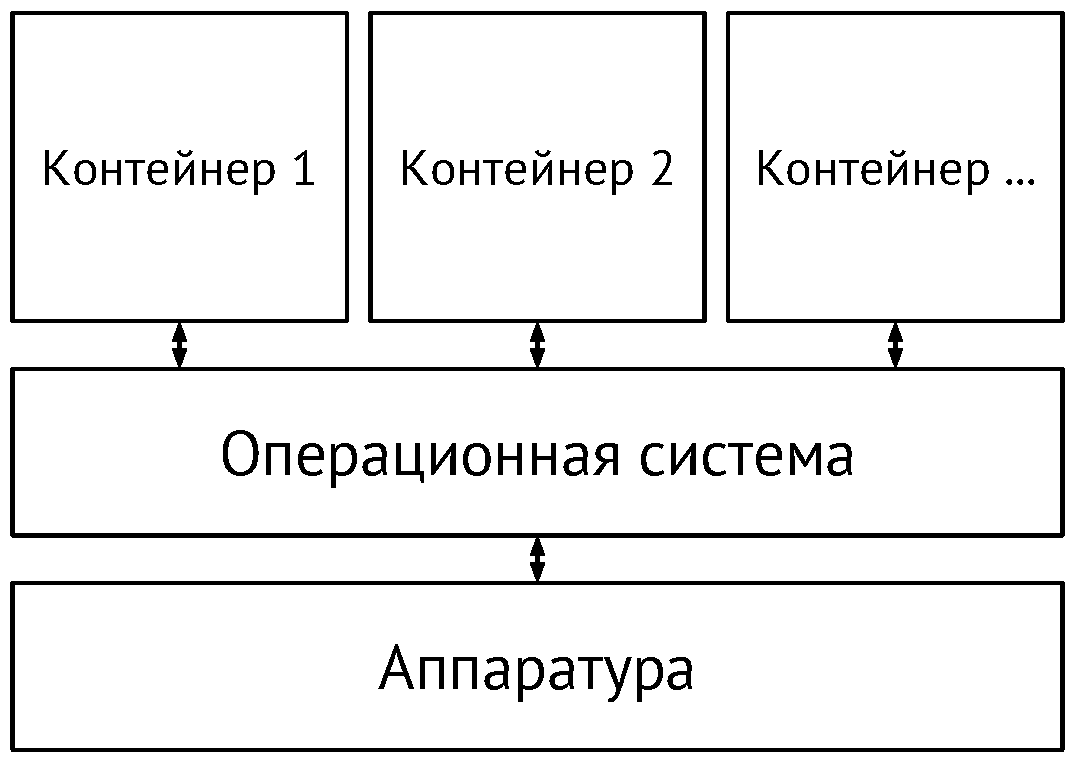
\includegraphics[width=\linewidth]{cont-virt} \\
		OpenVZ \pause \\
		\uncover<2->{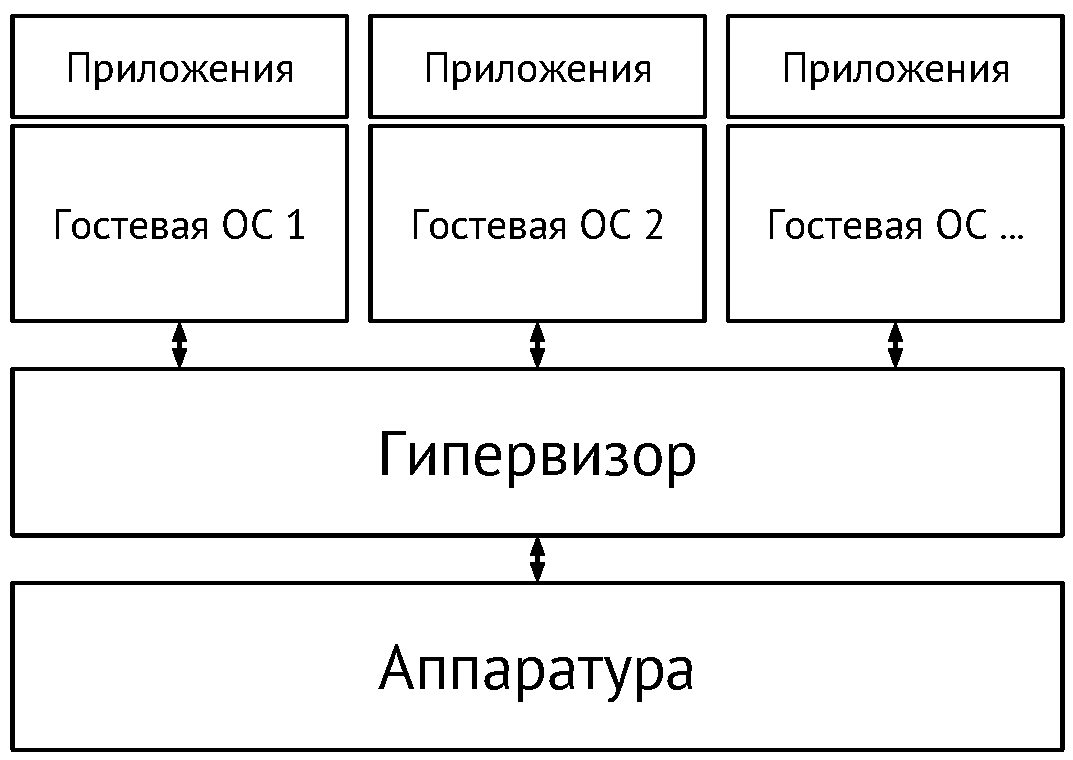
\includegraphics[width=\linewidth]{full-virt}}
		KVM
		\end{multicols}
	\end{center}
\end{figure}
\end{frame}

%-------------------------------------------------------------------------------

\section{Стек ПО для shared-хостинга}

\begin{frame}
\frametitle{\insertsection}
\framesubtitle{LAMP+Nginx (GPL/Apache), exim+dovecot+spamassasin+roundcube (GPL/LGPL/MIT)}
\begin{figure}[h]
	\begin{center}
		\begin{multicols}{2}
		
\includegraphics[width=\linewidth]{lamp} \\
		
\includegraphics[width=\linewidth]{mail}
		\end{multicols}
	\end{center}
\end{figure}
\end{frame}

%-------------------------------------------------------------------------------

\section{Резервное копирование}

\begin{frame}
\frametitle{\insertsection}
\framesubtitle{rsync (GPL)}
\begin{figure}[h]
	\begin{center}
		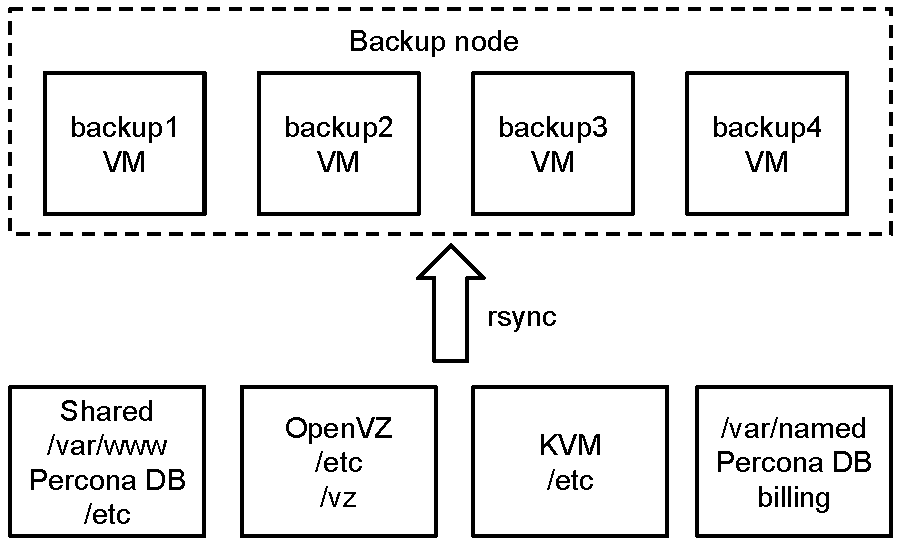
\includegraphics[width=\linewidth]{backup}
	\end{center}
\end{figure}
\end{frame}

%-------------------------------------------------------------------------------

\section{Вирусы и вредоносы}

\begin{frame}
\frametitle{\insertsection}
\framesubtitle{Linux Malware Detect (GPL)}
Возможности:
\begin{itemize}
	\item обнаружение вредоносов по хэш-сумме MD5
	\item отправка потенциально опасных файлов на сервис rfxn.com для внесения в базу сигнатур
	\item использование exclude-файлов
	\item удаление инфицированных base64 и gzinflate вставок
	\item перемещение зараженных файлов в карантин
	\item поиск по сигнатурам ClamAV
\end{itemize}
\end{frame}

%-------------------------------------------------------------------------------

\section{Защита сети}

\begin{frame}
\frametitle{\insertsection}
\framesubtitle{ddos-deflate (Artistic License) + IPTables/fail2ban/ipset (GPL)}
\begin{figure}[h]
	\begin{center}
		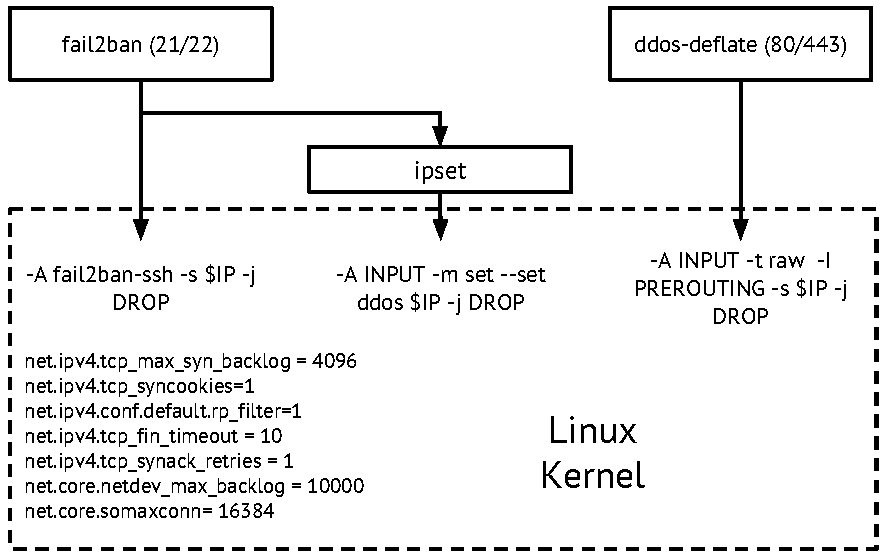
\includegraphics[width=\linewidth]{iptables}
	\end{center}
\end{figure}
\end{frame}

%-------------------------------------------------------------------------------

\section{Система отслеживания ошибок (bugtracker)}

\begin{frame}
\frametitle{\insertsection}
\framesubtitle{MantisBT (GPL)}
\begin{figure}[h]
	\begin{center}
		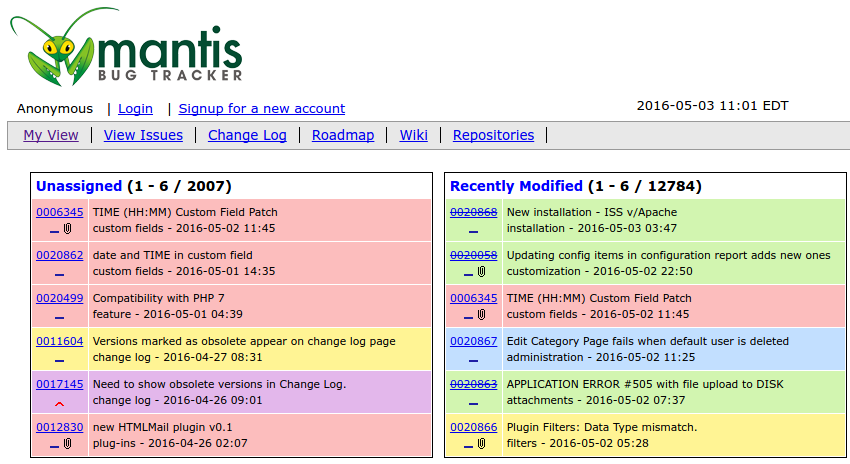
\includegraphics[width=\linewidth]{mantis}
	\end{center}
\end{figure}
\end{frame}

%-------------------------------------------------------------------------------

\section{Панели управления для клиентов}

\begin{frame}
\frametitle{\insertsection}
\framesubtitle{Vesta Control Panel (GPLv3)}
\begin{figure}[h]
	\begin{center}
		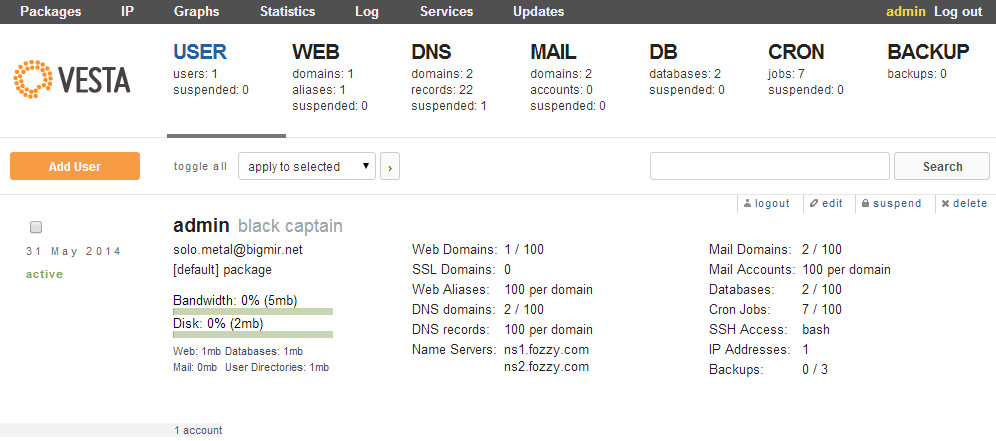
\includegraphics[width=\linewidth]{vesta}
	\end{center}
\end{figure}
\end{frame}

%-------------------------------------------------------------------------------

\section{Сравнение с закрытыми аналогами}

\begin{frame}
\frametitle{\insertsection}
\begin{figure}[h]
	\begin{center}
		\begin{tabular}{|l|p{7.5cm}|}
			\hline
			\bf{Open Source} & \bf{Closed Source} \\ \hline
			CentOS 7 & RHEL 7 --- \$900/год за 1 сервер \\
			Debian 8 & SLES 7 --- \$700/год за 1 сервер \\ \hline
			Nagios & Sensu --- \$2400/год за 100 серверов \\
			Munin & Opsview --- \$1870/год за 100 серверов \\ \hline
			OpenVZ & Virtuozzo --- \$6200/год за 100 контейнеров \\
			KVM & vCenter Server --- \$1750/год за 1 CPU \\ \hline
			Maldet & Virusdie --- \$20/год + \$2/год за сайт \\
			MantisBT & Jira --- \$6000 за 100 пользователей \\
			\hline
		\end{tabular}
	\end{center}
\end{figure}
\end{frame}

%-------------------------------------------------------------------------------

\section{Проекты в Open Source}

\begin{frame}
\frametitle{\insertsection}
\begin{itemize}
	\item openvz-tutorial (CC BY-SA 4.0): \href{https://github.com/Amet13/openvz-tutorial}{github.com/Amet13/openvz-tutorial}
	\item virtuozzo-tutorial (CC BY-SA 4.0): \href{https://github.com/Amet13/virtuozzo-tutorial}{github.com/Amet13/virtuozzo-tutorial}
	\item ddos-defalte (Artistic License 2.0): \href{https://github.com/Amet13/ddos-deflate}{github.com/Amet13/ddos-deflate}
	\item ansible-vz-wordpress (GNU GPLv3): \href{https://github.com/Amet13/ansible-vz-wordpress}{github.com/Amet13/ansible-vz-wordpress}
	\item icinga2-plugins-extra (GNU GPLv3): \href{https://github.com/Amet13/icinga2-plugins-extra}{github.com/Amet13/icinga2-plugins-extra}
	\item bachelor-diploma (CC BY-SA 4.0): \href{https://github.com/Amet13/bachelor-diploma}{github.com/Amet13/bachelor-diploma}
\end{itemize}
\end{frame}

%-------------------------------------------------------------------------------

\frame[plain]{\titlepage} % Титульный слайд
